\documentclass{article}
\usepackage[utf8]{inputenc}
\usepackage[L7x]{fontenc}
\usepackage[lithuanian]{babel}
\usepackage{lmodern}
\usepackage{amsmath}
\usepackage{graphicx}
\usepackage{verbatim}
\usepackage{hyperref}
\usepackage{subfigure}
\usepackage{tcolorbox}
\usepackage{framed}
\usepackage{mdframed}
\usepackage{tikz}
\usepackage{color}
\usepackage{cancel}
\usepackage[top=2cm, bottom=2cm, left=2cm, right=2cm, footskip=1cm, a4paper]{geometry}

\usepackage{hyperref}
\usepackage[upint]{stix}
\begin{document}
\section{Kaip įgyjamas matematikos supratimas?}

Šiame tekste remdamasis psichologijos žiniomis apie mąstymo procesą bei jo vystymosi raidą mėginsiu atsakyti į klausimą, kodėl moksleiviams ir studentams dažnai yra sunku pasiekti gerų rezultatų matematikoje ir kaip padidinti matematikos mokymosi efektyvumą.

\subsection{Moksleivių ir studentų sunkumų sprendžiant uždavinius pavyzdžiai}

Amerikiečių kolegijos dėstytojas M. Thornton (1984) aprašo reiškinį, kai kiekvienais metais į kolegiją įstoja keli studentai, pradiniuose kursuose visiškai nesuprantantys, kas vyksta matematikos paskaitose. Šie studentai neatrodo tingintys ar kvaili, kai kurie iš jų prie matematikos praleidžia labai daug laiko ir gerai išlaiko kitus dalykus. Atrodo, kad jiems mokantis kyla ne supratimas, o nusivylimas. Ši patirtis ypač pasimato studijuojant geometriją. Dėstytojas teigia būdamas pirmakursiu pats gavęs gerus pažymius daug atsimindamas, bet ne suprasdamas. Jis pripažino, jog būdamas antrakursiu nebuvo pasiruošęs deduktiniam samprotavimui, įrodymų ir aksiomomų supratimui, nes neturėjo tam reikiamų išvystytų mąstymo įgūdžių. Čia parodyta, kaip toje kolegijoje uždavinius sprendė kai kurie studentai.

\begin{framed}
\begin{enumerate}
\item \includegraphics[width=0.25\textwidth]{"similarity".png}

Abu pavaizduoti trikampiai yra panašūs. Raskite kraštinės $s$ ilgį.  

\textbf{Studento sprendimas:}$s \leftrightarrow 2, 7 \leftrightarrow 4, x \leftrightarrow 3$. Kadangi $2:4:3$, tai $s:7:x$ arba $5:7:6$. Vadinasi, $s=5$

\item Tarkime, kad jūsų mokytojui yra 40 metų, o jums 18 metų. Kiek procentų esate jaunesnis už savo mokytoją?

\textbf{Studento sprendimas:}$\frac{18}{40}=0.45\times 100=45\%$ jaunesnis.

\textbf{Kito studento sprendimas:}$\frac{40}{100}\times\frac{18}{x}=\frac{720}{100}=7.2\%$

\item Žiurkė, esanti tam tikrame labirinte, pereina kelią, sudarytą iš keturių išsišakojimų. Kiekviename išsišakojime ji gali pasirinkti tik sukti kairėn arba sukti dešinėn. Vienas iš šių kelių galėtų būti pažymėtas DDKK, kas reiškia, kad pirmąsyk žiurkė suks dešinėn, antrąsyk dešinėn, po to du kartus į kairę. Naudodami šį žymėjimą užrašykite visus kelius, kuriais galėjo eiti žiurkė

\textbf{Studento sprendimas:} KKKK, KKDD, KDKD, KKKD, KDDK, KDDD, DDKK, DKDK, DDDK, DKKD, DKKK, DDDD (12 kelių).
\end{enumerate}
\end{framed}

Uždaviniai, kuriuos pavyzdyje pateikė dėstytojas atitinka mūsų šalies vidurinio ugdymo programą. Aprašytą atvejį galiu papildyti panašiu atveju su moksleiviais, kuomet mokydamas vieną šeštoką matematikos uždaviau jam kelis klausimus.

\begin{framed}
\textbf{Pirmas pratimas mokiniui}. Atlik veiksmus su trupmenomis, kuriuos neseniai ėjote: $\frac{1}{3}+\frac{1}{5}$, $\frac{3}{7}+\frac{2}{7}$, $\frac{1}{2}\times \frac{1}{5}$.

\textbf{Mokinio sprendimas}.

\begin{enumerate}
\item $\frac{1}{3}+\frac{1}{5}=\frac{5}{15}+\frac{3}{15}=\frac{8}{15}$
\item $\frac{3}{7}+\frac{2}{7}=\frac{21}{49}+\frac{14}{49}=\frac{35}{49}$
\item $\frac{1}{2}\times \frac{1}{5}=\frac{5}{10}+ \frac{2}{10}=\frac{7}{10}$
\end{enumerate}

\textbf{Antras pratimas mokiniui}. Sugalvok tekstinį uždavinį, kuriame reikia dauginti du skaičius.

\textbf{Mokinio sprendimas}. Vienos mašinos greitis yra 60, kitos 140. Sudauginę gausime 8400.

\textbf{Signalinis klausimas}. Kur gyvenime tau prireikė naudoti daugybą?

\textbf{Mokinio atsakymas}. Neprireikė.

\textbf{Trečias pratimas mokiniui}. Kas įvyks, jei paveikslėlyje parodytą užtušuotą dalį padidinsime tris kartus? Pavaizduok tai sąsiuvinyje.

\textbf{Mokinio sprendimas}.

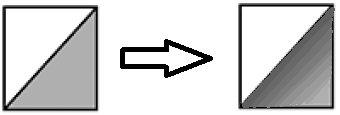
\includegraphics[width=0.4\textwidth]{density.png}
\end{framed}

Pagal pateiktus atvejus stengiantis išnagrinėti sunkumus, kylančius mokantis matematiką, tektų apsiriboti tik sunkumais, kylančiais mokantis mokyklinę programą. Studentams, besimokantiems matematiką Lietuvoje tokie pratimai būtų per lengvi, todėl vaizdžiai kalbant, nors šių pratimų analizė ir gali suteikti vertingų žinių apie matematikos mokymosi problemas, tačiau tai yra tik akiniai, skirti žiūrėti į tolį. Ji negali paaiškinti, kodėl turintys pakankamas kompetencijas studentai dažnai nepajėgia suprasti aukštosios matematikos teoremų, jų įrodymų ir dažnai pamiršta, kaip jas taikyti sprendžiant uždavinius.

\subsection{Mąstymo vystymosi vaidmuo matematikos ugdymo sistemoje}

Daugumos pasaulio šalių šiandienės mokyklinės matematikos ugdymo sistemos
susiklostė vykdant reformas, kurių pradžia siejama su ,,naująja matematika'' (angl. new math) vadinamu judėjimu. Praėjusio šimtmečio šeštame ir septintame dešimtmečiais vyko svarbūs pokyčiai Vakarų šalių ekonomikoje ir kultūroje. Buvo tikima, kad tolesniam eknominiam ir kultūriniam vystymuisi būtini aukštos kvalifikacijos darbuotojai ir mokslininkai. Kitas svarbus faktorius buvo konkurencija su tuometine Sovietų Sąjunga, kuri 1957 m. spalio 4 d. į kosminę erdvę sėkmingai paleido dirbtinį žemės palydovą. Baimė tapti technologiškai ir kariniu atžvilgiu atsilikusiomis valstybėmis paskatino jas peržiūrėti matematikos ir gamtos mokslų mokymą.

Antru svarbiu reformas paskatinusiu faktoriumi buvo pačios matematikos evoliucija. Grupė prancūzų matematikų, pasivadinusi
\textit{N. Bourbaki} slapyvardžiu, sugebėjo suvienyti atskiras matematikos sritis aibių teorijos pagrindu bei išplėtoti aksiomatinį metodą. Tai padėjo susiformuoti požiūriui į matematiką kaip į mokslo kalbą. Buvo tikima, kad matematika yra reikalinga visose srityse.

Trečias ,,naujosios matematiko'' judėjimo atsiradimo faktorius buvo pokyčiai pedagogikoje susiję su šveicarų psichologo
\textit{J. Piaget} darbais.  Jis įžvelgė analogiją tarp skaičiaus sąvokos formavimosi mechanizmo vaiko sąmonėje ir matematinių struktūrų.  Be to, Piaget akcentavo aktyvų mokymosi būdą, o \textit{N. Bourbaki} stiliaus matematika atrodė labai tam tinkama.
Šio darbo didžiąją dalį užims būtent šio psichologo idėjų aptarimas, praplėtimas ir pritaikymas.

Šveicaras Jeanas Piaget - vienas žymiausių XX a. raidos psichologų, pirmasis sistemingai tyrinėjęs kognityvųjį vystymąsi. Iki jo dauguma žmonių, užmiršę savo ikimokyklinius metus, manė, jog vaikai tiesiog mažiau žino, negu suaugusieji. Savo pirmajame darbe Piaget uždavinėjo vaikams klausimus, tikėdamasis nustatyti, kokio amžiaus vaikai gali atsakyti į pateiktus klausimus
teisingai. Jam kilo klausimas, kodėl vieno amžiaus vaikai negali atsakyti į tam tikrą klausimą, o teisingai atsakoį jį tik vėliau, būdami vyresni. Vėliau paaiškėjo, jog atsakymus į klausimus nulemia kognityvinė vaikų vystymosi raida. Psichologo nuomone, vaikas, pereidamas iš vienos su amžiumi susijusios stadijos į kitą, patiria pokyčių protrūkius, kuriuos seka stabilumo
periodai.  Kiekvienai stadijai būdingos skirtingos ypatybės, kurios lemia specifines mąstymo rūšis. Šios keturios stadijos yra:
\begin{itemize}
\item \textbf{Sensomotorinė stadija} (dažniausiai iki 2 m.). Pasaulis patiriamas pojūčiais ir veiksmais (žiūrint, liečiant, kramtant, sugriebiant)
\item \textbf{Priešoperacinė stadija} (maždaug nuo 2 iki 6 metų). Daiktus ženklina žodžiai ar vaizdai, bet logiškai nesamprotaujama.
\item \textbf{Konkrečių operacijų stadija} (maždaug nuo 7 iki 11 metų). Logiškai mąstoma apie konkrečius įvykius; suprantamos
konkrečios analogijos ir atliekamos aritmetinės operacijos.
\item \textbf{Formaliųjų operacijų stadija} (dažniausiai nuo 12 m.). Mąstoma abstrakčiai. Keliamos hipotezės, domimasi, kodėl tam tikri gamtoje esantys reiškiniai vyksta, imamas suvokti priežasties - pasekmės ryšys.

\end{itemize}
Šiuolaikiniai mokslininkai raidą laiko esant tolydesnę negu manė Piaget. Susipažinę su šiomis stadijomis aptarsime keletą į jo tyrimus įėjusių ir su vaikais atliktų uždavinių.

\begin{minipage}[b]{0.73\linewidth} 1. \textit{Iš pradžių ant stalo yra padėtos dvi vienodos stiklinės, kuriose yra po lygiai vandens ir viena, aukštesnė ir siauresnė, tuščia. Apklausėjas paklausia vaiko, ar jose yra po lygiai sulčių. Gavęs teigiamą atsakymą jis perpila iš pilnos stiklinės vandenį į tuščią ir pakartoja tą patį klausimą.} \end{minipage} \hspace{\fill} \begin{minipage}[b]{0.25\linewidth}\includegraphics[width=\textwidth]{"threecups".png} \end{minipage}\newline

\begin{minipage}[b]{0.79\linewidth} 2. \textit{Iš pradžių ant stalo yra padėtos dvi vienodos eilės monetų po penkias monetas. Apklausėjas paklausia vaiko, ar eilėse yra po lygiai monetų. Gavęs atsakymą jis antroje eilėje monetas perdeda taip, kad monetų išsidėstymas būtų platesnis ir pakartoja tą patį klausimą.} \end{minipage} \hspace{\fill} \begin{minipage}[b]{0.2\linewidth}\includegraphics[width=\textwidth]{"fivecoins".png} \end{minipage}\newline

3. \textit{Iš pradžių stalo pusėje, prie kurios sėdi vaikas, yra padėtas vienas sausainis, o kitoje pusėje du sausainiai. Apklausėjas paklausia vaiko ar tokios dalybos yra sąžiningos. Tada perlaužia vaiko pusėje esantį sausainį ir pakartoja klausimą.}

4. \textit{Mintinai atsakykite, kiek bus 4+5. Dabar mintinai atsakykite, kiek 9 - 5.}\newline

5. \textit{Mintinai atsakykite, kiek bus 3x+x?}

6. \textit{Birutė yra aukštesnė už Augustą, o Dominykas aukštesnis už Birutę. Kuris iš jų yra aukščiausias?}

7. \textit{Apklausos dalyviui, sėdinčiam prie stalo, duodame skirtingo ilgio siūlus, prie kurių galima pririšti skirtingo svorio daiktus ir paklausiame, nuo ko labiausiai priklauso švytuoklės svyravimo dažnumas: nuo siūlo ilgio, daikto svorio ar pradinio paleidimo greičio.}

Pirmose trijose situacijose apklausiami vaikai į pirmą klausimą atsako teisingai. Tačiau į antrą klausimą teisingai gebama atsakyti tik kognicijai pasiekus konkrečių operacijų stadiją. Priešoperacinės stadijos vaikams atrodys, kad trečioje stiklinėje sulčių yra daugiau, antroje eilėje monetų yra daugiau ir kad dalybos yra sąžiningos. Šiuos atsakymus jie paaiškina teiginiais ,,sulčių daugiau, nes stiklinė aukštesnė'', ,,monetų daugiau, nes jų eilė platesnė'' ir ,,dvi sausainio dalys yra tiek pat, kiek du sausainiai''. Iš šių eksperimentų galime suprasti, kad vaikai dažnai gali pastebėti tik vieną lyginamų objektų savybę (ilgį, plotį, kiekį, dydį), mano, kad keičiantis daikto formai, keičiasi ir jo kiekis. Ketvirta situacija parodo, kad priešoperacinėje stadijoje vaikai negali apgręžti atliekamos operacijos ir rezultatą 4 + 5 apskaičiuoti užtruks tiek pat laiko, kiek rezultatą 9 - 5. Įžengus į kitą stadiją atvirkčio veiksmo atlikimas bus suvoktas ir atsakymas gautas iškart.

Likę trys klausimai iliustruoja vaiko kognicijos perėjimą į formalių operacijų stadiją. Priešingu atveju į 5 klausimą atsakyti mintyse yra per sunku. Savo užsiėmimuose su moksleiviais ne kartą esu pastebėjęs, kad vaikas gali atsakyti tada uždavus konkretizuotą klausimą ,,Kiek bus 3 obuoliai + obuolys?'' ir paaiškinus, jog $x$ - tai bet kokio daikto ar dydžio žymėjimas. Į 6 klausimą mintinai pilnai atsakyti jis taip pat negali: jam reikia nusibraižyti vaikų ūgius popieriuje arba atsakymas gaunamas spėjimo būdu. Norint atsakyti į paskutinį klausimą, paprasčiausia yra pasirinkti bet kurį dydį (ilgį, svorį arba paleidimo greitį) ir jį pakeitus stebėti, ar pasikeičia dažnumas. Formalių opercijų stadijoje procesas atliekamas teisingai, o kitu atveju vaikai nėra tokie nuovokūs, dydžius keičia atsitiktine tvarka arba po kelis iš karto ir negali nustatyti teisingo atsakymo. 

Susipažinus su Piaget intektualinio vystymosi teorija, tampa aktualu, ar kognityviniai procesai gali būti paspartinti tinkamos mokomosios veiklos. Iš tiesų, pokyčiai tampa įmanomais tik tada, kai mokinys aktyviai sąveikauja su jį supančia fizine ir socialine aplinka, o darbas klasėje tėra to sąveikavimo dalimi. Tas pats atsakymas atsispindi ir Piaget (1964) pastebėjimuose: 

\textit{,,Nors patirtis yra būtina intelektualinio vystymosi dalis, tačiau galime atsidurti iliuzijoje, kad patirties suteikimas subjektui yra pakankamas jam atskirti struktūras. To nepakanka. Subjektas turi būti aktyvus, gebėti keisti daiktus ir atrasti struktūras savo paties sąveikoje su objektais.''}

\subsection{Kokių sugebėjimų trūksta mokantis mokyklinę matematiką}

Taikant kognityvinę vystymosį teoriją ikimokyklinukams ir kai kuriems pradinukams patariama jiems duoti pratimų, kuriuose
klasifikuojami įvairūs objektai ir užduoti nukreipiančius klausimus, pvz.,,kaip nusprendei, kokiai grupei
kiekvienas daiktas priklauso?'' arba ,,ar yra kitų būdų sugrupuoti daiktus?''. 

Remiantis pateikta teorija išaiškėja, kodėl referato pradžioje paminėtas šeštokas pateikė tokius atsakymus. Pirma, moksleivis buvo įsitikinęs, jog neatrado matematinių struktūrų, kuriose jam tektų susidurti su daugyba. Antra, jo suvokimas nebuvo pakankamas atskirti saryšiams tarp stebimų objektų savybių. Tą patvirtina du pavyzdžiai: pirma, moksleivis daugina du mašinos greičius, kai prasmę turi tik jų sudėtis ir lyginimas; antra, moksleivis painioja juslėmis suvokiamą ryškumo savybę su matematine figūros didumo savybe. Dėl panašių priežascių gerokai abstraktesni objektai, tokie kaip trupmenos, o tuo labiau jų saryšiai, moksleiviui bus nesuprantami. 

\subsection{Kokių sugebėjimų trūksta mokantis aukštąją matematiką}

Pavyzdys su studentais kol kas nėra tinkamas analizuoti remiantis Piaget tyrinėjimais tėra aišku, kad studentų
mastysena turi būti paskutiniame kognicijos etape, kas įvyksta apie 12-us metus. Tiesa, galima spėti, kad jie uždaviniuose pateiktų saryšių tarp matematinių objektų pilnai nesuprato todėl, kad besimokydami apie juos mokyklineje programoje
nebuvo pasiruošę mąstyti formaliai, del ko ir atsirado matematinės spragos. XXa. 8 - ajame dešimtmetyje atlikti psichologų tyrimai pagrindžia mąstymo įgūdžių trūkumo pasireiškimą ir suaugusių žmonių tarpe. Pastebėta, kad tik 50 - 60%
suaugusių žmonių tarp 25 - 30 metų, pagal kitų pratimų rodiklius pasiekę formalių operacijų stadiją praeina mūsų
nagrinėtą švytuoklės testą. 

Formalių operacijų stadijoje atsiranda sugebėjimai kelti prielaidas ir svarstyti apie galimas išvadas, leidžiantys
vaikui konstruoti savą matematiką. Be to, vaikai paprastai pradeda vystyti abstrakčius minčių modelius,
kuriuose samprotavimas vykdomas naudojant simbolius vietoj apčiuopiamų duomenų. Pavyzdžiui mokiniai gali
išspręsti lygtį x + 2x = 9 nesiremdami mokytojo padiktuota salyga kaip antai ,,Tomas suvalgė tam tikrą kiekį
saldainių, o jo sesė suvalgė du kartus daugiau. Abu kartu jie suvalgė 9 saldainius. Kiek saldainių suvalgė
Tomas?'' (Thornton, 1982). Samprotavimo įgūdžiai šioje stadijoje remiasi mentaliniais procesais, dalyvaujančiais
loginių argumentų apibendrinime ir įvertinime (Anderson, 1990). Trumpai apibūdinsime svarbiausias šių
procesų savybes.

\begin{itemize}
\item \textbf{Paaiškinimas} padeda moksleiviams atpažinti ir išnagrinėti uždavinio detales ir leidžia moksleiviams iššifruoti visą reikiamą informaciją, kurios prireiks sprendimui. Skatindami moksleivius išrinkti svarbią informaciją iš uždavinyje nurodytų teiginių mokytojai padeda jiems stiprinti matematinį supratimą.
\item \textbf{Gebėjimas kelti išvadą} skirstomas į dedukcinį ir indukcinį samprotavimą. Dedukcinis samprotavimas leidžia taikyti apibendrintas sąvokas ar taisykles konkretiems pavyzdžiams, o indukcinis - pastebėti konkrečių objektų ar įvykių panašumus ir skirtumus, išvesti jiems bendras taisykles.
\item \textbf{Įvertinimas} padeda moksleiviams nustatyti kriterijus, pagal kuriuos galima įvertinti sprendimo logiškumą. Mokytojai iš anksto apibrėžia taisykles, kuriomis remdamiesi moksleiviai gali nustatyti, ar sprendimas teisingas. Ši savybė reikalinga kelti prielaidoms apie būsimus įvykius ir svarstyti apie keliamų išvadų pagrįstumą.
\item \textbf{Pritaikymas} padeda moksleiviams sieti matematines sąvokas su realaus pasaulio pavyzdžiais. Vienas iš pavyzdžių galėtų būti racionaliosios lygties $\frac{1}{4}+\frac{1}{6}=\frac{1}{x}$ taikymas spęsti uždaviniui ,,Nepatyręs skynėjas vagą braškių nuskina per 6 valandas, o patyręs per 4. Per kiek laiko jie nuskins vagą kartu?''
\end{itemize}

\subsection{Kita}

Piaget's theory of intellectual development provides not only a very compelling model for
the description of reasoning skills but also a possible prescription for student growth. In his
article Piaget (1974) comments, ''My first conclusion is that learning of structures seems to obey
the same laws as the natural development of these structure. In other words, learning is
subordinated to development and not vice-versa.''

 The doctor's orders seem to be: If the symptoms of the mathematics student are those of
concrete operations we cannot treat him by working on the symptoms, that is by teaching
specific facts, concepts, methods. The cause must be treated. We must somehow change his level
of development before satisfactory learning of certain mathematics content will be possible.

 This prescription seems very difficult to take. It is much easier to restrict attention to
mathematical concepts from a course syllabus than to be concerned about a student's entire
intellectual capability. Discovering how a student reasons about a problem takes much more time
than asking if he has a correct answer. Time spent on reasoning processes will restrict,
sometimes severely, the amount of time available for mathematical content. An additional
complication is that usually a student's mathematics class is just a small part of his academic
load. Can one reasonably hope that what is done in one class will necessarily transfer to other
courses and to his life outside the university? 

\subsection{Šaltiniai}
\begin{enumerate}
\item \href{http://digitalcommons.unl.edu/cgi/viewcontent.cgi?article=1013\&context=adaptessays}{Melvin Thornton. Piagetian Programs in Higher Education}

\item \href{norvaisa.lt/wp-content/uploads/2012/07/laike-istriges-pasaulis.pdf}{Rimas Norvaiša. Matematikos mokymas - laike įstrigęs pasaulis}

\item \href{https://www.dropbox.com/s/vyghsx7k1ivd86g/David\%20G.\%20Myers\%20Psichologija\%202008.pdf?dl=0}{David G. Myers. Psichologija. 2008}

\item \href{https://pdfs.semanticscholar.org/3fbd/493c9bfa3d5a96bc2f82f8677b1de5b35b40.pdf\_ga=2.93207450.649401276.1573859970-917910527.1573859970}{Hyung Huh. A Piagetian experiment with the concrete - inquiry instruction model for acquisition and transfer of hypothetic-deductive scientific reasoning}

\item \href{https://files.eric.ed.gov/fulltext/EJ841568.pdf}{Bobby Ojose. Applying Piaget's Theory of Cognitive Development to Mathematics Instruction}
\end{enumerate}
\end{document}

